\documentclass[9pt,twocolumn,twoside]{../../styles/osajnl}
\usepackage{fancyvrb}
\usepackage{float}


\journal{i524} 

\title{AWS Lambda}

\author[1,*,+]{Karthick Venkatesan}


\affil[1]{School of Informatics and Computing, Bloomington, IN 47408, U.S.A.}


\affil[*]{Corresponding authors: vkarthickprabu@gmail.com}

\affil[+]{HID - S17-IO-3023}

\dates{paper1, \today}

\ociscodes{AWS Lambda,Serverless Computing, I524}

% replace this with your url in github/gitlab
\doi{\url{https://github.com/cloudmesh/sp17-i524/tree/master/paper2/S17-IO-3023/r
eport.pdf}}


\begin{abstract}
The rapid pace of innovation in data centers and the
software platforms within them is set to transform
how we build, deploy, and manage online applications
and services. Common to both hardware-based and container-based.
Virtualization is the central notion of a server. Servers
have been used for the past several years to back online applications, but new
cloud-computing platforms foreshadow the end of the
traditional backend server. Servers are notoriously difficult to configure and 
manage, and server
startup time severely limits an application’s ability to scale up and down 
quickly. As a result, a new model, called serverless computation, is poised to 
transform the construction of modern, scalable applications ability to
quickly scale up and down \cite{OpenLambda}. This paper is on AWS Lambda a 
Serverless Computing technology.
\end{abstract}

\setboolean{displaycopyright}{true}

\begin{document}

\maketitle

\section{Introduction}

Serverless applications are where some amount of server-side logic, unlike traditional architectures, is run in 
stateless compute containers that are event-triggered, ephemeral, and fully 
managed by a 3rd party. One way to think of this is ‘Functions as a service / 
Faas'. AWS Lambda is one of the most popular implementations of Faas 
\cite{www-Serverless}.


AWS Lambda is a FaaS(Function as a Service)  from Amazon Web Services. It runs 
the backend code on a high-availability compute infrastructure and performs all 
of the administration of the compute resources, including server and operating 
system maintenance and capacity provisioning \cite{www-CouchAWSLambda}.
 
In AWS Lambda one needs to pay only for the compute time consumed - there is no 
charge when the code is not running. AWS Lambda, can run code for virtually any 
type of application or backend service with zero administration. AWS 
Lambda requires only the code to be uploaded, and Lambda takes care of 
everything required to run and scale the code with high availability. AWS 
Lambda can be setup to automatically trigger the code from other AWS services 
or call it directly from any web or mobile app \cite{www-AWSLambda}.



\section{Features}

The key features of AWS Lambda are \cite{www-AWSLambda}
\begin{itemize}
\renewcommand{\labelitemi}{\scriptsize$\bullet$} 
\item \textbf{No Servers to Manage}: AWS Lambda automatically runs the code 
without requiring to provision or manage servers. Just write the code and 
upload it to Lambda.

\item \textbf{Continuous Scaling}: AWS Lambda automatically scales the 
application by running code in response to each trigger. The code runs in 
parallel and processes each trigger individually, scaling precisely with the 
size of the workload.

\item \textbf{Subsecond Metering}: With AWS Lambda, the institution using the 
service are charged for every 100ms the code executes and the number of times 
the code is triggered. They don't pay anything when the code isn't running.

\end{itemize}

\section{Architecture}

\begin{figure}[h]
\centering
\graphicspath{ {images/} }
\fbox{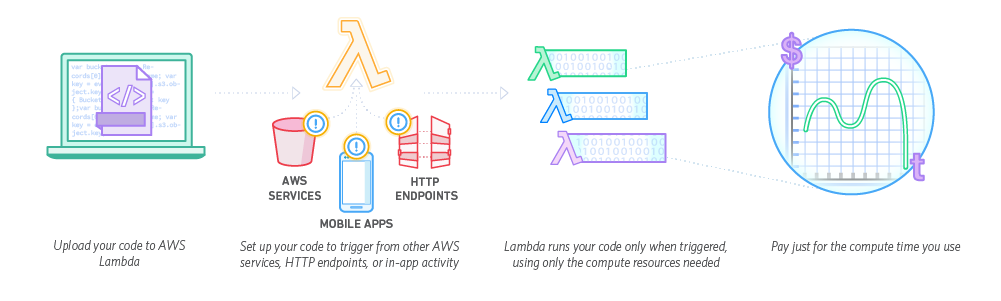
\includegraphics[width=\linewidth]{Lambda_HowItWorks}}
\caption{AWS Lambda Architecture} \cite{www-AWSLambda}
\label{fig:arch}
\end{figure}

Lambda functions and event sources are the core components in AWS Lambda. An 
event source is the entity that publishes events, and a Lambda function is the 
custom code that processes the events. Several AWS cloud services can be 
preconfigured to work with AWS Lambda. The configuration is referred to as 
event source mapping, which maps an event source to a Lambda function. It 
enables automatic invocation of Lambda function when events occur.

Each event source mapping identifies the type of events to publish and the 
Lambda function to invoke when events occur. The specific Lambda function then 
receives the event information as a parameter, and as shown in figure~\ref{fig:arch} the 
Lambda function code can then process the event.

The event sources can be any of the following:

\textbf{AWS services} – These are the supported AWS services that can be 
preconfigured to work with AWS Lambda. These services can be grouped as regular 
AWS services or stream-based services. Amazon Kinesis Streams 
\cite{www-AWSKinesis} and Amazon DynamoDB Streams \cite{www-AWSDynamoStream} 
are stream-based event sources, all others AWS services do not use stream-based 
event sources. 
 
\textbf{Custom applications} – Custom applications built can also publish 
events and invoke a Lambda function.

\section{Scalability}

\begin{figure}[H]
\centering
\graphicspath{ {images/} }
\fbox{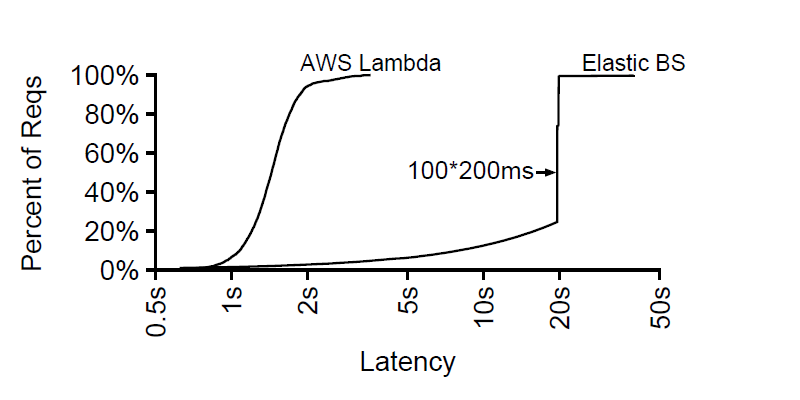
\includegraphics[width=\linewidth]{AWSLambdavsElasticBS}}
\caption{Response Time. This CDF shows measured
response times from a simulated load burst to an Elastic BS
application and to an AWS Lambda application.}  \cite{OpenLambda}
\label{fig:scale}
\end{figure}

A primary advantage of the Lambda model is its ability
to quickly and automatically scale the number of workers
when load suddenly increases. The Graph in figure~\ref{fig:scale} demonstrates this by 
comparing AWS Lambda to a container-based server platform,
AWS Elastic Beanstalk \cite{www-AWSEBS} (hereafter Elastic BS).
On both platforms, the same benchmark was run for one
minute: the workload maintains 100 outstanding RPC(Remote Procedure Calls)
requests and each RPC handler spins for 200ms.
Figure 2 shows the result: an RPC using AWS Lambda
has a median response time of only 1.6s, whereas an RPC
in Elastic BS often takes 20s. Investigating the cause for
this difference, it was found that while AWS Lambda was
able to start 100 unique worker instances within 1.6s to
serve the requests; all Elastic BS requests were served by
the same instance; as a result, each request in Elastic BS
had to wait behind 99 other 200ms requests.
AWS Lambda also has the advantage of not requiring
configuration for scaling. In contrast, Elastic BS con-
figuration is complex, involving 20 different settings for
scaling alone. Even though the Elastic BS was tuned to scale
as fast as possible, it still
failed to spin up new workers for several minutes  \cite{OpenLambda}.

\section{Documentation}

\begin{itemize}
\renewcommand{\labelitemi}{\scriptsize$\bullet$} 
\item Detailed documentation on AWS Lambda  Deployment , 
Configuration,Debugging and Development is available at \cite{www-AWSLambdaDoc}.
\item Use cases on reference architecture with  AWS Lambda are available at 
\cite{www-AWSLambdaUseCase}. 
\end{itemize}

\section{Competitors}

The main competitors for AWS Lambda are
\begin{itemize}
\renewcommand{\labelitemi}{\scriptsize$\bullet$} 
\item Microsoft Azure Functions
\item Google Cloud
\end{itemize}

A detailed comparison of features between AWS Lambda, Google Cloud and 
Microsoft Azure Functions is available in table~\ref{my-label}.

\begin{table*}[h]
\centering
\caption{AWS Lambda vs. Google Cloud Functions vs. Microsoft Azure Functions}
\cite{www-AWSLambdaCompareTable}
\label{my-label}
\renewcommand{\arraystretch}{1.25}%
\begin{tabular}{|p{3cm}|p{5cm}|p{4.5cm}|p{5.5cm}|}
\hline
\textbf{FEATURE} & \textbf{AWS LAMBDA} & \textbf{GOOGLE CLOUD} & \textbf{AZURE 
FUNCTIONS} \\ \hline
\begin{tabular}[c]{@{}l@{}}Scalability\\   \& availability\end{tabular} & 
Automatic scaling (transparently) & Automatic scaling & 
\begin{tabular}[c]{@{}l@{}}Metered scaling (App Service  Plan)\\ Automatic 
scaling (Consumption Plan)\end{tabular} \\ \hline
Max \# of functions & Unlimited functions & 20 functions per project (alpha) & 
Unlimited functions \\ \hline
Concurrent executions & 100 parallel executions (soft limit) & No limit & No 
limit \\ \hline
Max execution & 300 sec (5 min) & No limit & 300 sec (5 min) \\ \hline
Supported languages & JavaScript, Java Python, C\# & Only JavaScript & 
\begin{tabular}[c]{@{}l@{}}C\# and JavaScript (preview of  F\#,\\   Python, 
Batch, PHP, PowerShell)\end{tabular} \\ \hline
Dependencies & Deployment Packages & npm package.json & Npm, NuGet \\ \hline
Deployments & Only ZIP upload (to Lambda or S3) & 
\begin{tabular}[c]{@{}l@{}}ZIP upload, Cloud Storage or \\ Cloud  Source 
Repositories\end{tabular} & \begin{tabular}[c]{@{}l@{}}Visual Studio Team 
Services, OneDrive,\\  GitHub, Bitbucket, Dropbox\end{tabular} \\ \hline
Environment variables & Yes & Not yet & \begin{tabular}[c]{@{}l@{}}App Settings 
and ConnectionStrings \\from   App Services\end{tabular} \\ \hline
Versioning & Versions and aliases & Cloud Source branch/tag & Cloud Source 
branch/tag \\ \hline
Event-driven & \begin{tabular}[c]{@{}l@{}}S3, SNS, SES, DynamoDB, Kinesis,\\   
CloudWatch, Cognito, API Gateway\end{tabular} & 
\begin{tabular}[c]{@{}l@{}}Cloud Pub/Sub or Cloud Storage \\Object   Change 
Notifications\end{tabular} & \begin{tabular}[c]{@{}l@{}}Blob, EventHub, Generic 
WebHook \\  Queue, Http, Timer triggers\end{tabular} \\ \hline
HTTP(S) invocation & API Gateway & HTTP trigger & HTTP trigger \\ \hline
Orchestration & AWS Step Functions & Not yet & Azure Logic Apps \\ \hline
Logs management & CloudWatch & Cloud Logging & App Services monitoring \\ \hline
In-browser code editor & Yes & Only with Cloud Source Repositories & 
\begin{tabular}[c]{@{}l@{}}Functions environment, AppServices\\   
editor\end{tabular} \\ \hline
\begin{tabular}[c]{@{}l@{}}Granular\\   IAM\end{tabular} & IAM roles & Not yet 
& IAM roles \\ \hline
Pricing & \begin{tabular}[c]{@{}l@{}}1M requests for free (Free Tier), then\\   
\$0.20/1M requests\end{tabular} & Unknown until open beta & 
\begin{tabular}[c]{@{}l@{}}1 million requests and 400,000 GB-s\end{tabular} \\ 
\hline
\end{tabular}
\end{table*}


\section{Pricing}
With AWS Lambda, the users pay only for what they use. They are charged based 
on the number of requests for the functions and the duration the code executes. 

\textbf{Requests}: The users are charged for the total number of requests 
across all their functions. Lambda counts a request each time it starts 
executing in response to an event notification or invokes call, including test 
invokes from the console. First 1 million requests per month are free
\$0.20 per 1 million requests thereafter (\$0.0000002 per request)

\textbf{Duration}:Duration is calculated from the time the code begins 
executing until it returns or otherwise terminates, rounded up to the nearest 
100ms. The price depends on the amount of memory the user allocates to the 
function. The users are charged \$0.00001667 for every GB-second used 
\cite{www-AWSLambdaPricing}.

\section{Use Case}



\renewcommand{\labelitemi}{\scriptsize$\bullet$} 
\begin{figure}[H]
\centering
\graphicspath{ {images/} }
\fbox{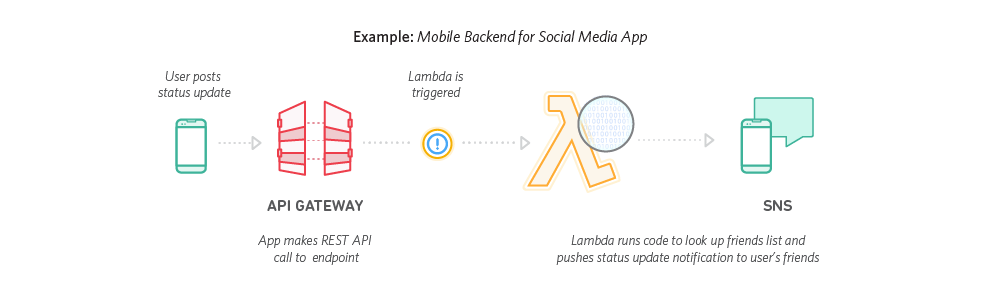
\includegraphics[width=\linewidth]{Mobile}}
\caption{Mobile Backend} \cite{www-AWSLambda}
\label{fig:usecase1}
\end{figure}

\textbf{Mobile Backends}: Mobile Backends are an excellent use case to 
implement AWS Lambda.As shown in figure~\ref{fig:usecase1} the backend of the mobile application 
can be built using AWS Lambda and Amazon API Gateway to authenticate and 
process API requests. Lambda makes it easy to create rich, personalised app 
experiences.
\textbf{Bustle.com} is a news, entertainment, lifestyle, and fashion website 
catering to women. Bustle also operates \textbf{Romper.com}, a website focused 
on motherhood.Bustle is based in Brooklyn, NY and is read by 50 million people 
each month. Bustle uses AWS Lambda to process high volumes of site metric data 
from Amazon Kinesis Streams \cite{www-AWSKinesis} in real time. This allows the 
Bustle team to get data more quickly so they can understand how new site 
features affect usage. They can also measure user engagement, allowing better 
data-driven decisions. The serverless back end supports the Romper website and 
iOS app as well as the Bustle iOS app. With AWS Lambda, Bustle was able to 
eliminate the need to worry about operations. The engineering team at Bustle 
focus on just writing code, deploy it, and it scales infinitely, and they don't 
have to deal with infrastructure management. Bustle was able to achieve the 
same level of operational scale with half the size of team of what is normally 
needed to build and operate the site  \cite{www-AWSLambdaBustle}.

\begin{figure}[H]
\centering
\graphicspath{ {images/} }
\fbox{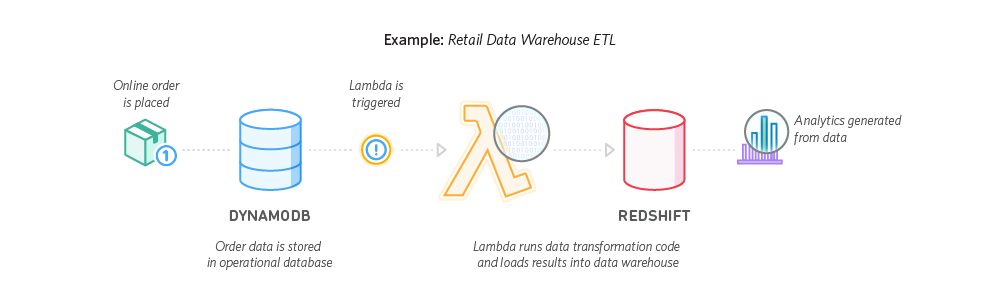
\includegraphics[width=\linewidth]{Lambda_ETL}}
\caption{Lambda ETL} \cite{www-AWSLambda}
\label{fig:usecase2}
\end{figure}

\textbf{Extract, Transform, Load}: As shown in figure~\ref{fig:usecase2} AWS Lambda can be used 
to perform data validation, filtering, sorting, or other transformations for 
every data change in a DynamoDB table and load the transformed data to another 
data store. \textbf{Zillow} is the leading real estate and rental marketplace 
dedicated to empowering consumers with data, inspiration and knowledge around 
the place they call home, and connecting them with the best local professionals 
who can help. Zillow needed to collect a subset of mobile app metrics in 
realtime and report it to the buisness users several times during the day.The 
solution was to be delivered in 3 weeks.Leveraging AWS Lambda and Amazon 
Kinesis Zillow was able to seamlessly scale 56 lines of code to over 16 million 
posts a day and achieve its goal in 2 weeks \cite{www-AWSLambdaZillow}.


\section{Conclusion}
Serverless Computing allows to build and run applications and services without 
thinking about servers. At the core of serverless computing is AWS Lambda, 
which lets to build auto-scaling, pay-per-execution, event-driven apps quickly.

\section*{Acknowledgements}

The authors thank Prof. Gregor von Laszewski for his technical guidance.
% Bibliography

\bibliography{references}


\end{document}
